\begin{figure*}[h!]
\centering
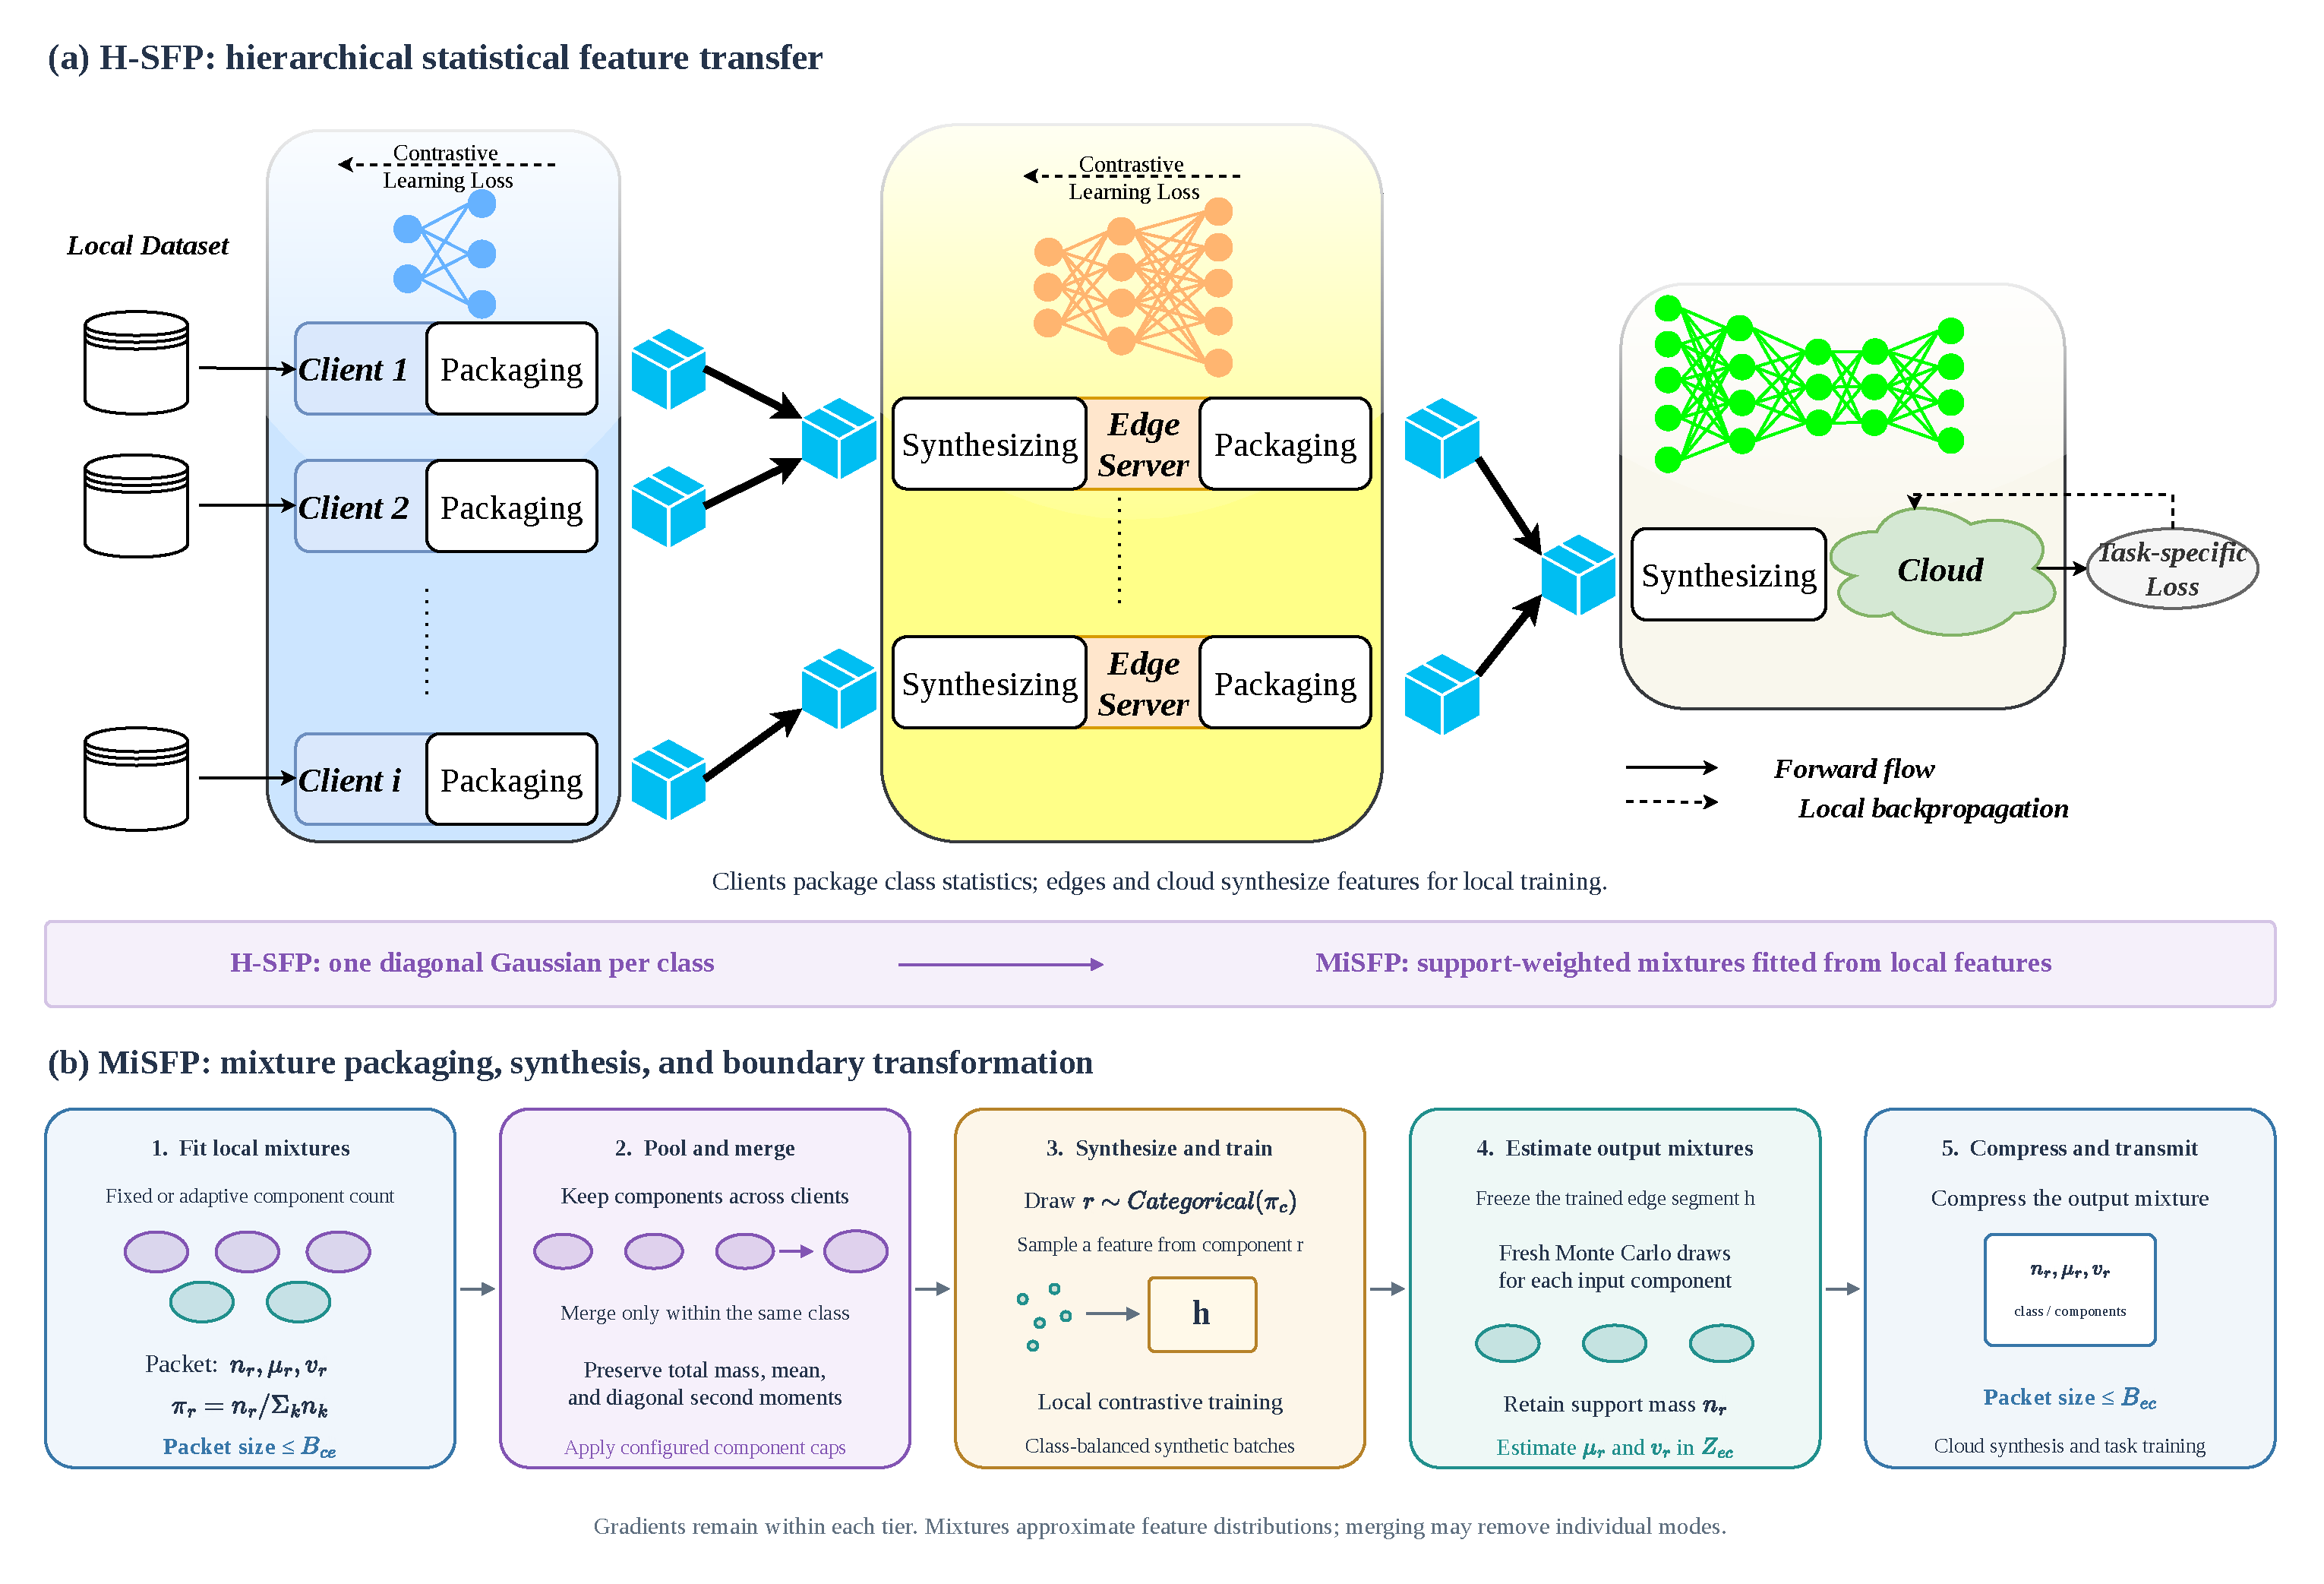
\includegraphics[width=\textwidth]
{figures/misfp_architecture.pdf}
\caption{Statistical feature transfer across clients,
edges, and the cloud.
(a) H-SFP~\cite{tran2026h} generates upper-tier training
inputs from single-Gaussian class summaries.
Solid arrows indicate forward flow; dashed arrows
indicate local backpropagation.
(b) MiSFP constructs and compresses mixtures, trains
the edge from synthetic features, re-estimates
output-space statistics, and compresses the outgoing
packet for cloud training.
Step~4 illustrates the default \emph{propagate} mode,
which retains incoming component support masses.}
\label{fig:architecture}
\end{figure*}
\section{MiSFP}
\label{sec:method}

H-SFP trains successive model segments from synthetic
features generated using single-Gaussian class
summaries~\cite{tran2026h}.
MiSFP uses support-weighted mixtures to retain multiple
components within and across clients.
Its execution comprises local mixture construction,
class-wise pooling and compression, synthetic edge
training, output-space re-estimation, and cloud training
(Fig.~\ref{fig:architecture}).
Gradients remain within the segment being optimized;
parameter synchronization is performed separately.

\subsection{Local Training and Mixture Construction}

Mixture statistics are estimated in the raw,
unnormalized feature spaces defined in
\cref{sec:problem}.
Contrastive similarities and cloud prediction use
the stabilized normalization
\begin{equation}
\label{eq:normalization}
\operatorname{norm}_{\epsilon_n}(\bm r)
=
\frac{\bm r}{\max\{\|\bm r\|_2,\epsilon_n\}},
\qquad \epsilon_n>0.
\end{equation}
The normalization floor is fixed, and the cloud applies
the same normalization during training and inference.
Communicated moments are computed before normalization.

Client $i$ trains its encoder using supervised
contrastive learning~\cite{khosla2020supervised}.
Let $\mathcal A$ index a batch and define
$\bm q_a=\operatorname{norm}_{\epsilon_n}(\bm r_a)$
for raw representation $\bm r_a$.
The positive set is
$\mathcal P(a)=
\{p\in\mathcal A\setminus\{a\}:y_p=y_a\}$,
and $\mathcal A_+$ contains the anchors with
nonempty positive sets.
The objective is
\begin{equation}
\label{eq:supervised_contrastive}
\begin{aligned}
\mathcal L_{\mathrm{SC}}
&=
-\frac{1}{|\mathcal A_+|}
\sum_{a\in\mathcal A_+}
\frac{1}{|\mathcal P(a)|}
\sum_{p\in\mathcal P(a)}
\log\rho_{ap},\\
\rho_{ap}
&=
\frac{\exp(\bm q_a^\top\bm q_p/\tau)}
{\sum_{b\in\mathcal A\setminus\{a\}}
 \exp(\bm q_a^\top\bm q_b/\tau)},
\end{aligned}
\end{equation}
with $\tau=0.1$.
Classification batches contain two augmented views
of each image.
Anchors without positives are excluded, and an update
is skipped if no valid anchors remain.

After local training, the encoder is fixed for feature
extraction.
Nonfinite feature vectors are discarded and counted.
Classification uses embeddings after encoder pooling;
segmentation uses labeled spatial embeddings
(Section~\ref{subsec:segmentation}).

For each represented class, seeded k-means++
initialization and Lloyd iterations determine
component centers.
Center fitting may use a reservoir of at most
4096 features.
Assignment counts and population moments nevertheless
use every valid feature in the corresponding fitting set.
Each component stores a support mass and two
length-$d$ moment vectors, giving
$\mathcal O(Kd)$ parameter storage for $K$ components.
Although each component has diagonal covariance,
differences between component means allow the mixture
to exhibit cross-coordinate dependence.

Fixed variants request $K\in\{1,2,4\}$ components.
For $K>1$, every component must satisfy the configured
minimum support, whose default is $s_{\min}=3$.
If this condition fails, fitting is repeated with
a smaller $K$.
A nonempty class can fall back to one component even
when its total support is below $s_{\min}$.
Thus, this support condition constrains multi-component
fitting; it does not suppress small nonempty classes.

Adaptive construction selects $K$ for each
client--class pair.
For classification, a seeded split reserves 30\%
of valid class features for validation.
Client-side segmentation uses image-disjoint subsets.
Let $\mathcal V_{ic}$ denote the validation features
and $q_{ic}^{(K)}$ a candidate density fitted without
using those features.
Feasible candidates are scored by
\begin{equation}
\label{eq:component_selection}
\begin{aligned}
\mathcal J_{ic}(K)
&=
-\frac{1}{d_{ce}|\mathcal V_{ic}|}
\sum_{z\in\mathcal V_{ic}}
\log q_{ic}^{(K)}(z)+\lambda(K-1),
\end{aligned}
\end{equation}
for $K\in\{1,\ldots,K_{\max}\}$.
Likelihood evaluation uses a positive variance floor.
The default configuration uses $K_{\max}=4$,
$\lambda=0$, and at least four validation features.
A minimizing candidate with $K>1$ is accepted only if
$
\mathcal J_{ic}(1)-\mathcal J_{ic}(K)>\delta,
$
where $\delta=0.02$ nat/dimension by default.
When a positive penalty is configured, the required
unpenalized NLL improvement is
$\delta+\lambda(K-1)$.
Insufficient validation data or support yields $K=1$.
The selected mixture is refitted on all valid class
features, with support checks applied again.

This selector is a local density-fit heuristic;
it does not directly optimize the receiving model's
predictive loss.
Fixed and adaptive allocations are therefore evaluated
as separate configurations in \cref{sec:experiments}.
Table~\ref{tab:variants} distinguishes local component
requests from hierarchical retention.
Experiment-specific overrides are reported with
the evaluation settings.

\begin{table}[t]
\caption{Default MiSFP component requests and per-class
retention limits.
Support checks can reduce the local request.
For the non-K1 variants, the regular edge-input cap
is unset and a safety cap of 32 is configured.
``--'' denotes no explicit cap.
Optional byte budgets can further reduce retention.}
\label{tab:variants}
\centering
\small
\setlength{\tabcolsep}{4pt}
\begin{tabularx}{\columnwidth}{@{}Xcccc@{}}
\toprule
Variant
& Local
& Edge
& Edge
& Cloud\\
& $K$
& input
& output
& pool\\
\midrule
K1       & $1$    & $1$  & $1$ & $1$\\
Edge     & $1$    & $32$ & $4$ & --\\
K2       & $2$    & $32$ & $4$ & --\\
K4       & $4$    & $32$ & $4$ & --\\
Adaptive & $\leq4$ & $32$ & $4$ & --\\
\bottomrule
\end{tabularx}
\end{table}

\begin{algorithm}[t]
\caption{Client packet construction}
\label{alg:client}
\begin{algorithmic}[1]
\Require features by class, selection settings,
         $s_{\min}$, optional budget $B_{ce}$
\For{each locally represented class $c$}
    \State discard and count nonfinite features;
           skip the class if none remain
    \State select $K$ using the fixed request or
           \eqref{eq:component_selection}
    \State refit on all valid class features;
           reduce $K>1$ if support checks fail
    \State compute
           $(n_{icr},\bm\mu_{icr},\bm v_{icr})$
           from all final assignments
\EndFor
\State apply same-class compression under $B_{ce}$
       if configured
\State serialize the packet; report infeasibility
       if the budget cannot be met
\end{algorithmic}
\end{algorithm}
\subsection{Pooling and Budgeted Merging}

A receiving tier concatenates compatible components
separately by class
(Fig.~\ref{fig:architecture}(b), Step~2).
Pooling and pair comparisons are performed within
one boundary feature space, subject to the compatibility
checks in \cref{sec:problem}.
Local component indices do not identify corresponding
modes across sources.

For two same-class components with positive masses
$a$ and $b$, the pooled parameters are
\begin{align}
m
&=a+b,
\qquad
\bm\mu=
\frac{a\bm\mu_a+b\bm\mu_b}{m},
\label{eq:poolmean}\\
\bm v
&=
\frac{a}{m}
\left[\bm v_a+(\bm\mu_a-\bm\mu)^2\right] +
\frac{b}{m}
\left[\bm v_b+(\bm\mu_b-\bm\mu)^2\right].
\label{eq:poolvar}
\end{align}
Squares are elementwise.
These expressions preserve the total mass, mean,
and coordinate-wise second moments of the represented
components in exact arithmetic
(\cref{sec:analysis}).

Candidate pairs are scored by
\begin{equation}
\label{eq:mergecost}
\Delta(a,b)
=
\frac{ab}{a+b}
\left(
\|\bm\mu_a-\bm\mu_b\|_2^2
+
\|\sqrt{\bm v_a}-\sqrt{\bm v_b}\|_2^2
\right).
\end{equation}
The parenthesized term is the squared
$2$-Wasserstein distance between the two diagonal
Gaussians.
The support factor incorporates their masses into
the pair ranking.
This does not equal the distance between
the mixtures before and after merging.

Compression first enforces the configured per-class
caps by repeatedly merging the admissible pair with
the smallest $\Delta$.
If an outgoing packet still exceeds its byte budget,
additional same-class merges minimize $\Delta$
divided by the positive reduction in complete
serialized size.
For fixed-size component records and an unchanged
header, each merge saves the same number of bytes,
so this ranking reduces to the ranking by $\Delta$.
Canonical component ordering resolves ties
deterministically.

The optional budgets $B_{ce}$ and $B_{ec}$ apply
to outgoing client and edge packets, including metadata.
Receiver-side pools are governed separately by their
component caps.
At least one component remains for every represented
class.
If the minimum class-preserving packet exceeds the
budget, compression reports infeasibility under the
configured warning or error policy. Feasibility is determined from the serialized packet size.
The procedure provides deterministic component reduction
under the configured constraints.
Its moment identities do not guarantee optimal compression.
Figure~\ref{fig:merging} shows the process.

\begin{figure}[t]
\centering
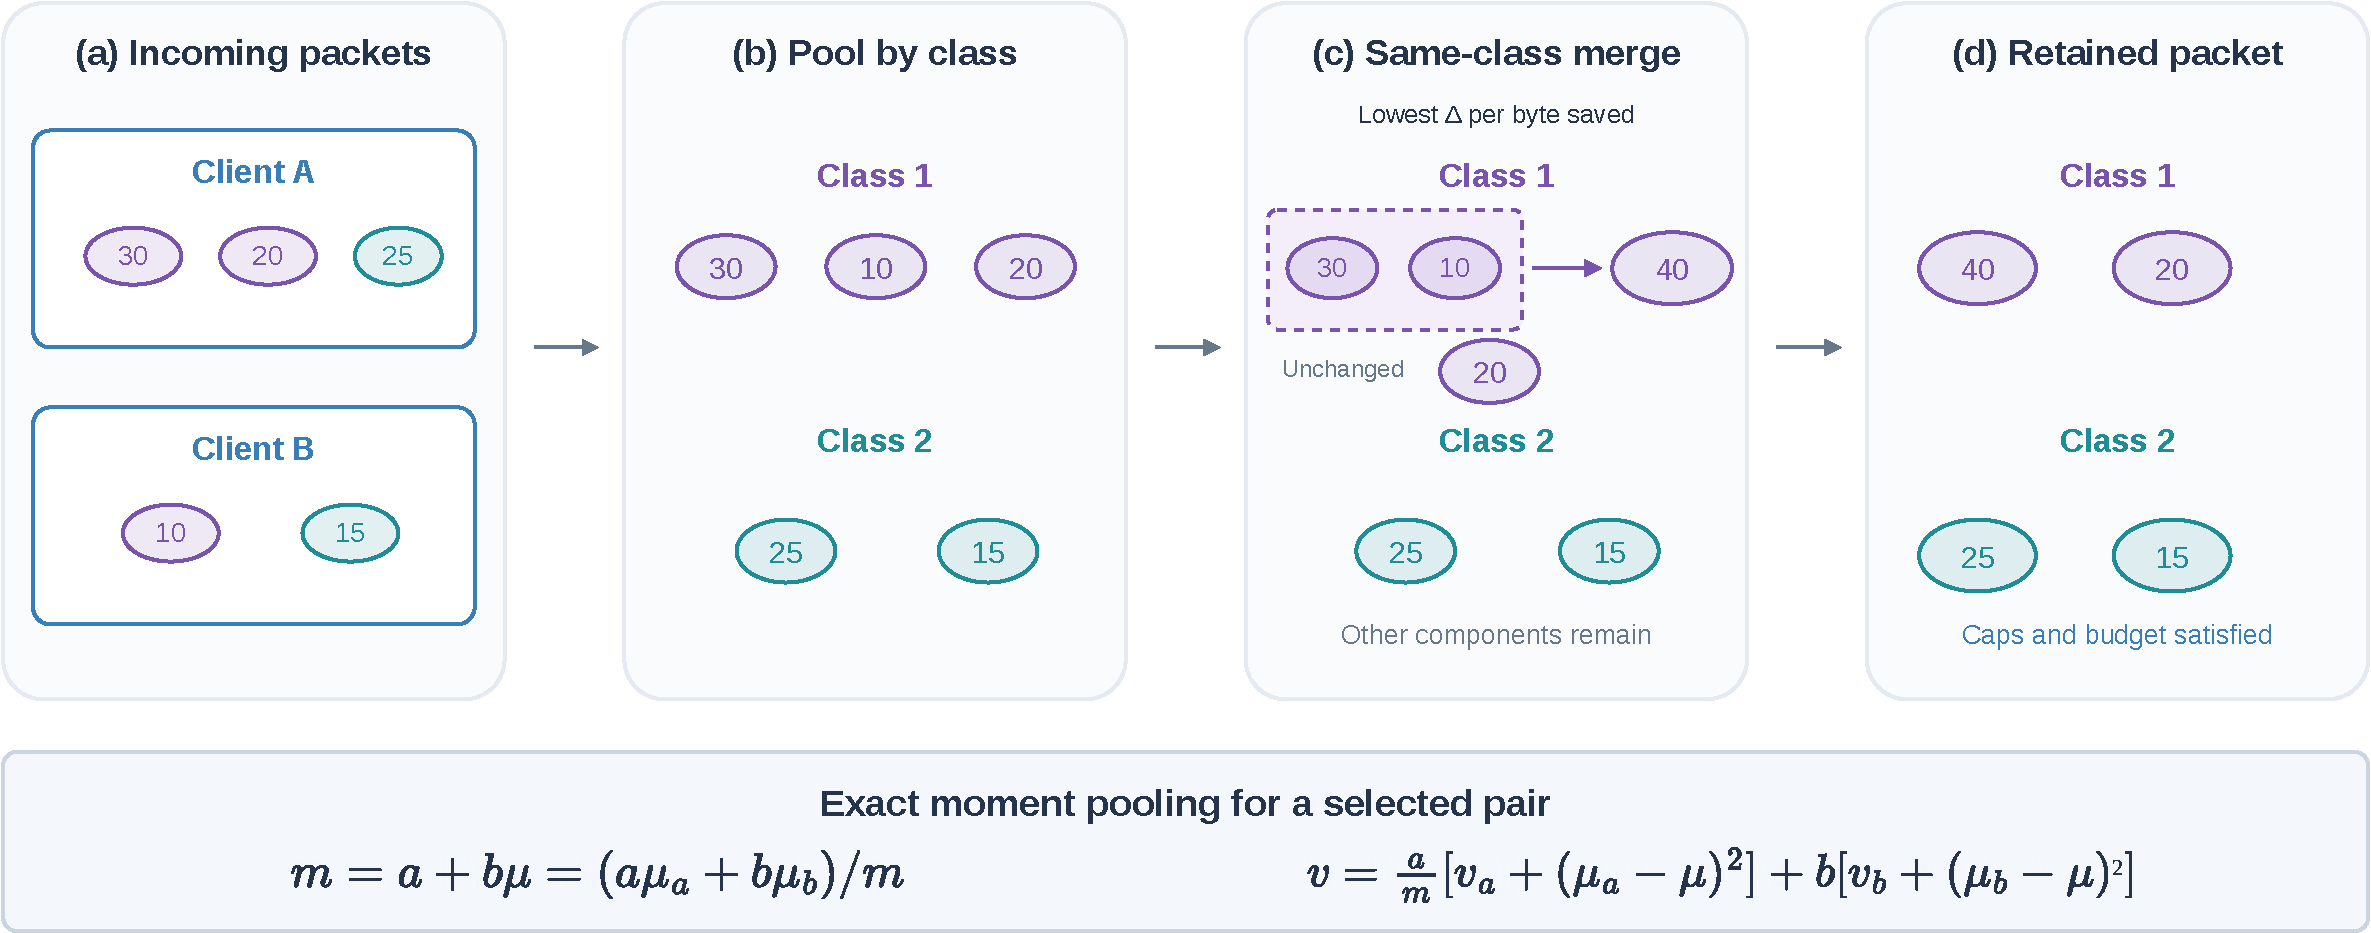
\includegraphics[width=\columnwidth]
{figures/misfp_merging.pdf}
\caption{Class-preserving pooling and compression.
Colors denote classes and numbers denote component
support masses.
Same-class merges preserve aggregate mass, means,
and coordinate-wise second moments in exact arithmetic.
The $\Delta$-per-byte criterion applies during
byte-budget compression.}
\label{fig:merging}
\end{figure}

\subsection{Synthesis and Nonlinear Boundary Transformation}

For a retained class mixture $Q_c$, let $\bm\pi_c$
contain its normalized component masses.
MiSFP first draws
$r\sim\mathrm{Categorical}(\bm\pi_c)$
and then generates
\begin{equation}
\label{eq:mixture_sampling}
\tilde z
=
\bm\mu_{cr}
+
\sqrt{\max(\bm v_{cr},\epsilon_s)}
\odot\bm\xi,
\qquad
\bm\xi\sim\mathcal N(\bm 0,I),
\end{equation}
where $\epsilon_s>0$, and the maximum and square root
are elementwise.
A balanced synthesis schedule supplies $M_c$ features
per represented class, while within-class sampling
follows the support weights.
Stored variances remain unfloored during construction
and merging; floors are applied only during
likelihood evaluation and sampling.

The edge trains $h_{\theta_e}$ from raw synthetic
inputs using \eqref{eq:supervised_contrastive}
on normalized edge outputs.
Each selected class contributes at least two synthetic
features per batch.
The received mixture statistics remain fixed
during this optimization.

After training, the edge fixes $h_{\theta_e}$
and estimates summaries in its raw output space.
A nonlinear map generally transforms a Gaussian
into a non-Gaussian distribution.
Consequently, the input parameters cannot simply
be reused in $\mathcal Z_{ec}$.
MiSFP supports two finite-sample estimation modes.

In the default \emph{propagate} mode
(Fig.~\ref{fig:architecture}(b), Step~4),
the edge draws a fixed number of fresh Monte Carlo
samples from each retained input component,
using 50 samples per component by default.
The transformed samples determine one output mean
and population diagonal variance per input component.
Each output retains its incoming support mass.
Equal sampling effort therefore does not make
the mixture weights uniform.

In \emph{refit} mode, the edge draws
$M_c^{\mathrm{bd}}$ fresh features from the complete
class mixture and transforms them through $h_{\theta_e}$.
This boundary-estimation count is configured separately
from the training sample count and defaults to
200 features per class.
The outputs are reclustered using the configured
output-component selection rule.
Each output component receives its assignment fraction
multiplied by the incoming class support, yielding
a potentially noninteger effective mass.

Both modes approximate the transformed sampling
distribution.
The output components are compressed under
the edge-output cap and optional $B_{ec}$.
Algorithm~\ref{alg:edge} shows the operation.

\begin{algorithm}[t]
\caption{Edge receive--train--emit operation}
\label{alg:edge}
\begin{algorithmic}[1]
\Require compatible client packets, component caps,
         optional budget $B_{ec}$, estimation mode
         and sample counts
\State concatenate received components by class
\State apply configured caps to the pooled input
\State sample class-balanced features using
       \eqref{eq:mixture_sampling}
\State train $h_{\theta_e}$ using
       \eqref{eq:supervised_contrastive}, then fix it
\If{mode is \emph{propagate}}
    \For{each retained input component}
        \State draw and transform the configured
               number of fresh Monte Carlo samples
        \State estimate output moments;
               retain the incoming support mass
    \EndFor
\Else
    \State draw and transform
           $M_c^{\mathrm{bd}}$ features per class
    \State refit output mixtures; assign effective
           masses from assignment fractions
           and incoming class support
\EndIf
\State compress under the output cap and optional $B_{ec}$
\State serialize the packet; report infeasibility
       if the budget cannot be met
\end{algorithmic}
\end{algorithm}

\subsection{Cloud Training and Model Synchronization}
\label{subsec:training}

The cloud pools compatible edge-output components
by class, applies any configured component cap,
and synthesizes a class-balanced training set
in $\mathcal Z_{ec}$.
The head $g_{\theta_g}$ applies
\eqref{eq:normalization} followed by a linear classifier
and is trained using cross entropy,
$
\ell_{\theta_g}(s,c)
=
-\log[\operatorname{softmax}(g_{\theta_g}(s))]_c
$.
The same normalization is applied to real features
during inference.
Morover, parameter synchronization follows two intervals.
Every $t_1$ rounds, each edge averages the latest
encoder update from every client that participated
during the preceding window.
Each client contributes once, weighted by its
training-dataset size.
The resulting encoder is broadcast to all attached
clients; an edge without updates retains its
previous checkpoint.
Every $t_2$ rounds, the cloud separately averages
edge-level encoder checkpoints and edge-segment
parameters, weighting edge $e$ proportionally to
$N_e=\sum_{i\in\mathcal C_e}|\mathcal D_i|$.
The aggregated encoder and edge segment are broadcast
through the hierarchy, while the cloud head remains
central.
The synchronization schedule uses $t_1=5$
and $t_2=10$.

Synchronization follows the round's training updates.
Within-edge aggregation precedes global aggregation
when both are due.
Subsequent packets identify their extraction model version, although periodic synchronization does not ensure coordinate alignment between locally updated encoders.
Total communication includes mixture packets and
parameter exchanges.
Matched H-SFP and MiSFP comparisons use the same
training objectives, task architectures, and
synchronization schedule.
MiSFP-K1 remains a separate control because it uses
the mixture packet path and moment-pooling operator.

\subsection{Application to Semantic Segmentation}
\label{subsec:segmentation}

For segmentation, the client retains the 128-channel
spatial feature map produced by ResNet-18 through
layer~2.
Ground-truth masks are resized to this grid using
nearest-neighbor interpolation.
Valid spatial embeddings are grouped by pixel label to construct foreground and background mixtures.
Component support counts the embeddings assigned to each one. Additionally, the edge applies a $1\times1$ convolution from 128 to 256 channels followed by ReLU, and the cloud uses a pointwise two-class head.
The client encodes spatial context; the upper-tier
mappings operate on individual embeddings.
Normalization in \eqref{eq:normalization} is applied
across channels at each location, allowing these
mappings to train on synthesized
features.

Client training applies~\eqref{eq:supervised_contrastive} to labeled spatial embeddings~\cite{wang2021pixelcontrast}.
Geometric augmentations are applied consistently to images and masks. Adaptive client construction uses image-disjoint fitting and validation subsets, followed by a final refit using all eligible local training features.
Aggregation is weighted by counts, separately from pixel-component masses.

Edge and cloud training use the synthetic-feature procedure above, with contrastive and pixelwise cross-entropy objectives, respectively.
During inference, the model preserves
the spatial feature grid.
Two-class logits are bilinearly upsampled to the
original image resolution before classwise argmax.
Foreground IoU and Dice are evaluated on complete
predicted masks.